%%%%%%%%%%%%%%%%%%%%%%%%%%%%%%%%%%%%%%%%%%%%%%%%%%%%%%%%%%%%%%%%%%%%%%%%
\chapter{Ungoliant: The Second OSCAR pipeline}
%%%%%%%%%%%%%%%%%%%%%%%%%%%%%%%%%%%%%%%%%%%%%%%%%%%%%%%%%%%%%%%%%%%%%%%%

\begin{center}
    \begin{minipage}{0.66\textwidth}
        \begin{small}
            In which we present the work of \citet{abadji-etal-2021-ungoliant}, who after the evaluations discussed in the previous two chapters, completely rewrote the original OSCAR's \goclassy pipeline, added features to the corpus such as metadata extraction and published the second version of the OSCAR corpus now known as OSCAR 21.09.
        \end{small}
    \end{minipage}
    \vspace{0.5cm}
\end{center}


As discussed in previous chapters, OSCAR 2019 was generated from the plain text data extracts (WET files) of the November 2018 Common Crawl dump, which was distributed in the form of 56,000 \emph{shards}, that were then filtered and classified by language \citep{ortiz-suarez-etal-2019-asynchronous,ortiz-suarez-etal-2020-monolingual}. OSCAR 2019 is now available for research through the Huma-Num servers \footnote{\url{https://oscar-corpus.com/post/oscar-2019/}} in Europe and for the public at large through Hugging Face's Datasets Hub \footnote{\url{https://huggingface.co/datasets/oscar}} where it now has more than 15 thousands downloads.

OSCAR 2019 came in four different versions, each one intended for different tasks. These versions were either \emph{unshuffled} or \emph{shuffled} (that is, for each language, lines have been shuffled, destroying record and thus document integrity), and \emph{non-deduplicated} or \emph{deduplicated} (since duplicate lines account for more than half of the total data\footnote{OSCAR-orig: 6.3TB, OSCAR-dedup: 3.2TB} generated by the pipeline). For the unshuffled versions, each language file contained paragraphs that came from the same record, and each paragraph is separated by a newline.

Simply put, OSCAR 2019 was composed of single language files that contained textual data (\texttt{ta.txt} for the Tamil language, for example). However, due to the often huge sizes of these files, and subsequently the impracticality of storage and distribution, OSCAR 2019 files were split and compressed in equally sized parts.

However, but OSCAR 2019 and its pipeline came with a number of limitations, which we will discuss in the following sections, and we will try to start fixing in this and the following chapter.

\section{Limitations of the OSCAR 2019 Corpus and its Generation Pipeline}

\subsection{OSCAR 2019}

OSCAR 2019 was inherently linked to its generation pipeline, and as such its quality partly depended on the pipeline's quality. While OSCAR 2019 was considered to be one of the cleanest multilingual corpora available \citep{caswell-etal-2020-language,kreutzer-etal-2021-quality}, several problems had been described, and the state of the publicly available code raised questions about maintenance and maintenability of the pipeline itself.

Apart from the fact that its content dated back to 2018, OSCAR 2019 corpus suffered from quality issues already discussed in chapter \ref{chap:quality} and of course more in depth in \citep{caswell-etal-2020-language,kreutzer-etal-2021-quality}, some of which include:

\begin{itemize}
    \item \textbf{Language label mismatches and inconsistencies}, which occurs earlier in the pipeline and would be fixable downstream,
    \item \textbf{Representation washing} as defined by \citet{kreutzer-etal-2021-quality}, whereby low resource languages, while present in the corpus, are of a significantly lower quality than higher resource languages without any quality metric available publicly.
\end{itemize}

Moreover, the more recent dumps of Common Crawl in 2021 contain more than 64,000 shards (almost 10,000 more than the dump used for OSCAR 2019). Furthermore, each of these shards is composed of numerous records, and each record holds textual content along with metadata. While Common Crawl shards hold document-level metadata that could be useful downstream, they were com discarded and do not appear in OSCAR 2019, whereas other corpora generated from Common Crawl do include them, e.g.~CCNet \citep{wenzek-etal-2020-ccnet}. This limits OSCAR 2019 users to the textual content only, whereas metadata could have been distributed along with the corpus itself.

\subsection{goclassy}

OSCAR 2019 was built using \goclassy, a high-performance asynchronous pipeline written in Go \citep{ortiz-suarez-etal-2019-asynchronous}. However, it suffered from several caveats that makes the re-generation and update of the corpus relatively complex in practice.

While \goclassy's source code was easily readable thanks to the choice of an uncluttered programming language and a pragmatic approach, the lack of structure in both the source and the project itself made \goclassy difficult to extend and maintain.

The pipeline was not functional out-of-the-box, as the user had to provide the compressed shards from CommonCrawl, manually install FastText \citep{joulin-etal-2016-fasttext,joulin-etal-2017-bag} and create specific directories by themselves, since only partial instructions are given in the supplied README file.

\goclassy also made heavy use of I/O, as data was saved and loaded repeatedly between steps; as an example, the identification step stored language identification data and individual sentences in two files, before generating the final files (one per language). Despite these limitations, \goclassy's performance remained acceptable mainly due to Go's emphasis on easy and efficient parallelization and inherent speed. The pipeline for instance used clever handling of file descriptors and employed extensive buffering, which limited I/O calls cost in some parts.

\section{Building a New Version of the OSCAR Corpus}

Having identified some shortcomings of both OSCAR 2019 and its pipeline, \goclassy, we decided to restart the OSCAR project by completely rewriting our pipeline. To that end, we introduce \emph{Ungoliant}, a new corpus generation pipeline that, like \goclassy, creates a large-scale multilingual text corpus from a Common Crawl dump. However, contrarily to \goclassy, Ungoliant is fully modular, better structured, and highly parametrizable; thereby allowing comparisons between several parallelization strategies. A specific effort was put in testing and documentation. Parts of Ungoliant are heavily inspired by \goclassy, although for its implementation we decided to use Rust rather than Go, which is often considered to be a faster more low level programming language.\footnote{\url{https://benchmarksgame-team.pages.debian.net/benchmarksgame/fastest/rust-go.html}}

We also use Ungoliant to generate a new version of the OSCAR corpus from a more recent Common Crawl dump. The new corpus includes metadata information while retaining backward compatibility with the OSCAR 2019 corpus.


\subsection{Ungoliant}

\subsubsection{Rationale and Scope}
\label{subsubsec:rationale}
While Ungoliant is heavily inspired by \goclassy, it provides a better set of tools to download, process, filter and aggregate textual and contextual data from Common Crawl. These operations can be sequential, parallel or both, depending on contexts and performance requirements.

We provide both batch and streaming processing, so that the whole pipeline could be run either online, with every step running on streams of data, or offline, with every step running on tangible files, or a mix of both, using already downloaded Common Crawl dumps but streaming the rest of the process. Moreover, we embed numerous filtering and deduplication utilities directly inside Ungoliant, making these features available for pipeline composition and post-processing.

Ungoliant features a loosely defined pipeline interface, on which we re-implement \goclassy's one, while improving performance by threading more aggressively and avoiding I/O where it is not necessary: While \goclassy uses intermediate files for tags and sentences, we try to keep everything in memory in order to avoid losing time loading or writing files. The Rust language provides constructs that helps us build complex abstractions and pipelines while limiting proactive file I/O or computing, since nearly all the reimplemented pipeline is built around lazy evaluation. File I/O is only used when loading shards, and when writing sentences in language files.

Through benchmarking we found that the best parallelization strategy is to use rayon\footnote{\url{https://github.com/rayon-rs/rayon}}, a work-stealing \cite{blumofe-etal-1999-scheduling} parallel and concurrent library enabling massive parallelization. We parallelize on \mbox{shard-,} record- and sentence-level processing.

To evaluate Ungoliant performance, we run both \goclassy and Ungoliant's implementation on 1, 10, 25 and 100 Common Crawl shards both on a middle-range laptop computer (i5-7200u, 8GB RAM, NVMe SSD) and a HPC node (Xeon 5218 (64 Threads), 180GB RAM). Results are shown in Table~\ref{tab:goclassy-bench}.

\begin{table}[t]
    \centering\small
    \scalebox{0.85}{
        \begin{tabular}{lrrrr}
            \toprule
            Platform                 & \#shards & goclassy & Ungoliant & Approx.~speedup \\
            \midrule
            \multirow{3}{*}{Desktop} & 1        & 30s      & 13s       & $\times$2.3     \\
                                     & 10       & 3m6s     & 2m12s     & $\times$1.3     \\
                                     & 25       & 9m10s    & 5m47s     & $\times$1.5     \\
            \midrule
            \multirow{3}{*}{HPC}     & 1        & 40s      & 6s        & $\times$6.6     \\
                                     & 25       & 2m40s    & 1m6s      & $\times$2.4     \\
                                     & 100      & 7m59s    & 4m14s     & $\times$1.8     \\
            \bottomrule
        \end{tabular}
    }
    \caption{Comparison of approximate generation times depending on platform and number of shards.}
    \label{tab:goclassy-bench}
\end{table}

Ungoliant performs better than \goclassy on all tasks, independently of the platform or number of shards processed. However, we can note that Ungoliant's speedup is higher on short tasks, which is explained by its aggressive multithreading strategy, while \goclassy uses a record-scope multithreading at its finest granularity.


\subsection{Iterating on the goclassy Pipeline}


Common Crawl dumps contain metadata that hold useful information such as related records, recognized language(s), or origin URLs. Since OSCAR's 2019 pipeline discarded metadata and sentences could be shuffled, we lost the ability to investigate the metadata itself, as well as working on potentially multilingual documents, since we separated text from metadata.

The new pipeline (and the resulting new corpus schema) aims to establish a first link between textual data and metadata from Common Crawl, while staying backward compatible with the existing OSCAR 2019 schema.

In other words, switching from the original OSCAR 2019 corpus and the newly generated one should be a drop-in operation.

% début ajout explication extraction metadata
\subsubsection{Metadata Extraction and Linking}
Our choice of keeping the corpus backward compatible with the original OSCAR 2019 introduces changes in the way the corpus is generated, namely regarding metadata: a record's body is composed of sentences that \textbf{aren't guaranteed to be of the same language}. Since OSCAR merges sentences from multiple records into a single file, special attention has to be paid to the metadata dispatch too.

Approaches to tackle this problem range from (1) storing all metadata in a single location to (2) having language-specific metadata files that contain the metadata for each line in the language file.

Both (1) and (2) have their strengths and weaknesses, namely:
\begin{enumerate}
    \item Having all metadata at the same place may facilitate wide queries about whole metadata, but at a cost of a very large size (which harms both accessibility and performance).
    \item Getting the metadata for a given line is fast since line numbers are synchronized, but there is repeated information and a potentially important increase in size.
\end{enumerate}

We thus choose a hybrid approach which keeps metadata local to each language, while trying to limit the information repetition by keeping an entry by group of \emph{chunks} rather than by line, where a \emph{chunk} is a series of contiguous sentences that share the same language from the same document.

An overview of the pipeline can be seen in Figure~\ref{fig:zoomed}, where we depict Ungoliant at a macro level in the first part of the figure, and where we also give a more precise view on record processing and metadata extraction in the second half of the figure.

Metadata is distributed via JSON-encoded files holding an ordered list of metadata entries, along with offsets ($o$) and paragraph lengths ($l$), enabling any user to get the content of a said metadata by querying for lines $(o, o+l]$ in the content file.

This approach still has drawbacks, in particular when looking for the corresponding metadata of a given sentence/paragraph, where one has to perform a search on the metadata file, or when working with multilingual documents. Another important drawback is the resulting cost of potentially merging back numerous language parts: Since metadata query is offset-based, merging back metadata files implies updating those offsets.

\begin{figure*}
    \centering
    \begin{tikzpicture}[auto,scale=0.85, every node/.style={transform shape},font=\sffamily]
        \tikzstyle{nod}=[minimum width=1.65cm,minimum height=6cm,rectangle,rounded corners=10pt,
        fill=red!20, align=center, text width=1.65cm,text centered]
        \tikzstyle{ft} = [minimum width=1.5cm,minimum height=1cm,rectangle,rounded corners=10pt,
        fill=blue!20, align=center, text width=1.5cm,text centered]
        \tikzstyle{fin}=[minimum width=4cm,minimum height=4cm,rectangle,rounded corners=10pt,
        fill=green!20, align=center, text width=4cm,text centered]
        \tikzstyle{arr}=[->,>=stealth,thick]
        \tikzstyle{arr1}=[->,>=stealth,thick]

        \node[nod] (CC) at (0,0) {Common Crawl};

        \node[minimum width=2cm, text width=2cm,text centered] (TEX1) at (2.5,3.45) {\small Compressed Files};
        \node (GZ1) at (2.5,2.3) {\Huge \faFileArchive};
        \node (GZ2) at (2.5,1) {\Huge \faFileArchive};
        \node (GZ3) at (2.5, -0.3) {\Huge \faFileArchive};
        \node (DGZ) at (2.5, -1.2) {\Huge $\vdots$};
        \node (GZ4) at (2.5,-2.3) {\Huge \faFileArchive};


        \node[minimum width=1cm, text width=1cm,text centered] (TEX1) at (4.5,3.45) {\small WET Files};
        \node (T1) at (4.5,2.3) {\Huge \faFile};
        \node (T2) at (4.5,1) {\Huge \faFile};
        \node (T3) at (4.5, -0.3) {\Huge \faFile};
        \node (DT) at (4.5, -1.2) {\Huge $\vdots$};
        \node (T4) at (4.5,-2.3) {\Huge \faFile};

        \node[ft] (F1) at (7,2.3) {Process Record};
        \node[ft] (F2) at (7,1) {Process Record};
        \node[ft] (F3) at (7,-0.3) {Process Record};
        \node (DF) at (7, -1.2) {\Huge $\vdots$};
        \node[ft] (F4) at (7,-2.3) {Process Record};

        \node[minimum width=2.3cm, text width=2.3cm,text centered] (TEX1) at (10.25,3.45) {\small Metadata, Paragraph, Language Tag};
        \node (TA1) at (10.25,2.3) {\faCode $\,$ \faParagraph $\,$ \faTags};
        \node (TA2) at (10.25,1) {\faCode $\,$ \faParagraph $\,$ \faTags};
        \node (TA3) at (10.25, -0.3) {\faCode $\,$ \faParagraph $\,$ \faTags};
        \node (DTA) at (10.25, -1.2) {\Huge $\vdots$};
        \node (TA4) at (10.25,-2.3) {\faCode $\,$ \faParagraph $\,$ \faTags};


        \node[minimum width=2.3cm, text width=2.3cm,text centered] (TEX1) at (15,3.45) {\small Files Classified by Language};
        \node[fin] (FF) at (15,0) {};
        \node (TF) at (15,1.3) {\Huge \faLanguage $\,\cdots$\faLanguage};
        \node (TF3) at (15, 0) {\Huge \faLanguage $\,\cdots$\faLanguage};
        \node (TF3) at (15, -1.3) {\Huge \faLanguage $\,\cdots$\faLanguage};


        \draw[arr] (1,2.3)--(GZ1);
        \draw[arr] (1,1)--(GZ2);
        \draw[arr] (1,-0.3)--(GZ3);
        \draw[arr] (1,-2.3)--(GZ4);


        \draw[arr] (GZ1)--(T1);
        \draw[arr] (GZ2)--(T2);
        \draw[arr] (GZ3)--(T3);
        \draw[arr] (GZ4)--(T4);


        \draw[arr1] (5,2.5)--(6.1,2.5);
        \draw[arr1] (5,2.3)--(6.1,2.3);
        \draw[arr1] (5,2.1)--(6.1,2.1);

        \draw[arr1] (5,1.2)--(6.1,1.2);
        \draw[arr1] (5,1)--(6.1,1);
        \draw[arr1] (5,0.8)--(6.1,0.8);

        \draw[arr1] (5,-0.1)--(6.1,-0.1);
        \draw[arr1] (5,-0.3)--(6.1,-0.3);
        \draw[arr1] (5,-0.5)--(6.1,-0.5);

        \draw[arr1] (5,-2.1)--(6.1,-2.1);
        \draw[arr1] (5,-2.3)--(6.1,-2.3);
        \draw[arr1] (5,-2.5)--(6.1,-2.5);


        \draw[arr] (8,2.5)--(9.1,2.5);
        \draw[arr] (8,2.3)--(9.1,2.3);
        \draw[arr] (8,2.1)--(9.1,2.1);

        \draw[arr] (8,1.2)--(9.1,1.2);
        \draw[arr] (8,1)--(9.1,1);
        \draw[arr] (8,0.8)--(9.1,0.8);

        \draw[arr] (8,-0.1)--(9.1,-0.1);
        \draw[arr] (8,-0.3)--(9.1,-0.3);
        \draw[arr] (8,-0.5)--(9.1,-0.5);

        \draw[arr] (8,-2.1)--(9.1,-2.1);
        \draw[arr] (8,-2.3)--(9.1,-2.3);
        \draw[arr] (8,-2.5)--(9.1,-2.5);


        \draw[arr] (TA1.0)--(FF);
        \draw[arr] (TA2.0)--(FF);
        \draw[arr] (TA3.0)--(FF);
        \draw[arr] (TA4.0)--(FF);
    \end{tikzpicture}
    %\caption{A scheme of the \emph{goclassy} pipeline. The red square represents the Compressed WET files stored on Amazon Web Services. The {\faFileArchive} icons represent the gzip files stored locally, the {\faFile} represent one of the 64K WET files. The {\faFile} represents the filtered file and the {\faTags} represents a file of language tags, one tag per line in \faFileTextO. The {\faLanguage} represents one of the 166 classified files. Each arrow represents an asynchronous non blocking worker and dotted arrows represent a line filtering process.}
    % \captionsetup{singlelinecheck=off}
    % \caption{
    % Scheme of the Ungoliant pipeline. The red square represents CommonCrawl content hosting, where the compressed shards are fetched. The \textit{Process Shard} steps hold shard processing, paragraph creation and merging (see Figure~\ref{fig:zoomed}), and are internally parallelized.
    % \label{fig:overview}
    % \begin{itemize}
    %     \item \faFileArchive : CommonCrawl compressed shard.
    %     \item \faFile : Uncompressed shard, containing records.
    %     \item \faCode : Record Metadata 
    %     \item \faTag : Language identification 
    %     \item \faParagraph : Paragraph, composed of sentences identified as \faTag
    % \end{itemize}
    % }



    \tikzset{every picture/.style={line width=0.75pt}} %set default line width to 0.75pt        

    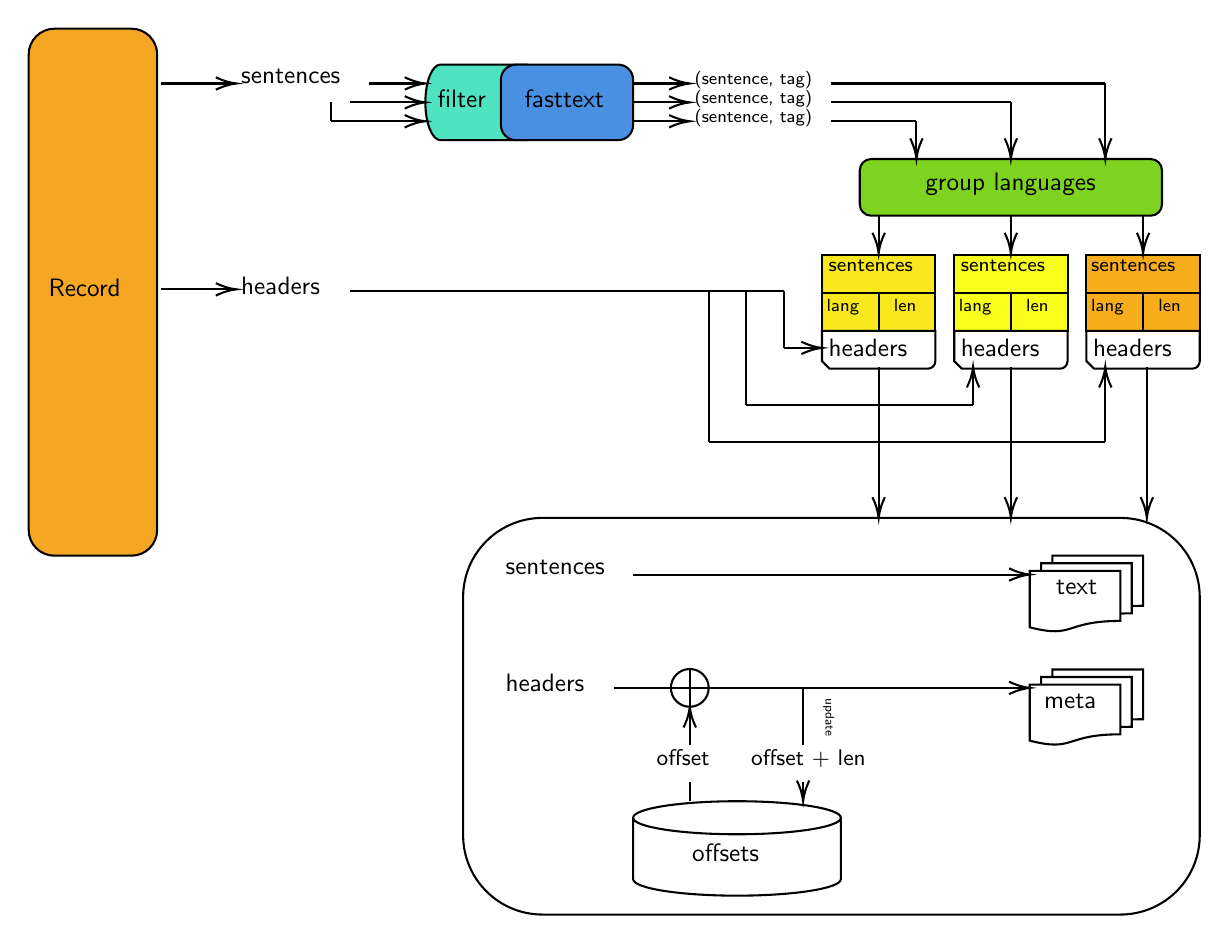
\begin{tikzpicture}[x=0.75pt,y=0.75pt,yscale=-0.91,xscale=0.91, every node/.style={scale=0.91}, font=\sffamily]
        %uncomment if require: \path (0,489); %set diagram left start at 0, and has height of 489

        %Flowchart: Stored Data [id:dp4699321019986179] 
        \draw  [fill={rgb, 255:red, 80; green, 227; blue, 194 }  ,fill opacity=1 ] (238,30) -- (280,30) .. controls (275.58,30) and (272,38.95) .. (272,50) .. controls (272,61.05) and (275.58,70) .. (280,70) -- (238,70) .. controls (233.58,70) and (230,61.05) .. (230,50) .. controls (230,38.95) and (233.58,30) .. (238,30) -- cycle ;
        %Rounded Rect [id:dp4628690629420654] 
        \draw  [fill={rgb, 255:red, 245; green, 166; blue, 35 }  ,fill opacity=1 ] (20,24.6) .. controls (20,17.09) and (26.09,11) .. (33.6,11) -- (74.4,11) .. controls (81.91,11) and (88,17.09) .. (88,24.6) -- (88,276.4) .. controls (88,283.91) and (81.91,290) .. (74.4,290) -- (33.6,290) .. controls (26.09,290) and (20,283.91) .. (20,276.4) -- cycle ;
        %Straight Lines [id:da8313420982420904] 
        \draw    (90,40) -- (128,40) ;
        \draw [shift={(130,40)}, rotate = 180] [color={rgb, 255:red, 0; green, 0; blue, 0 }  ][line width=0.75]    (10.93,-3.29) .. controls (6.95,-1.4) and (3.31,-0.3) .. (0,0) .. controls (3.31,0.3) and (6.95,1.4) .. (10.93,3.29)   ;
        %Straight Lines [id:da4482967760350627] 
        \draw    (90,149) -- (128,149) ;
        \draw [shift={(130,149)}, rotate = 180] [color={rgb, 255:red, 0; green, 0; blue, 0 }  ][line width=0.75]    (10.93,-3.29) .. controls (6.95,-1.4) and (3.31,-0.3) .. (0,0) .. controls (3.31,0.3) and (6.95,1.4) .. (10.93,3.29)   ;
        %Rounded Rect [id:dp9849601809689044] 
        \draw  [fill={rgb, 255:red, 74; green, 144; blue, 226 }  ,fill opacity=1 ] (270,38) .. controls (270,33.58) and (273.58,30) .. (278,30) -- (332,30) .. controls (336.42,30) and (340,33.58) .. (340,38) -- (340,62) .. controls (340,66.42) and (336.42,70) .. (332,70) -- (278,70) .. controls (273.58,70) and (270,66.42) .. (270,62) -- cycle ;

        %Straight Lines [id:da8668621904345621] 
        \draw    (200,40) -- (228,40) ;
        \draw [shift={(230,40)}, rotate = 180] [color={rgb, 255:red, 0; green, 0; blue, 0 }  ][line width=0.75]    (10.93,-3.29) .. controls (6.95,-1.4) and (3.31,-0.3) .. (0,0) .. controls (3.31,0.3) and (6.95,1.4) .. (10.93,3.29)   ;
        %Straight Lines [id:da996242982187254] 
        \draw    (180,50) -- (180,60) ;
        %Straight Lines [id:da7644452497572334] 
        \draw    (190,50) -- (228,50) ;
        \draw [shift={(230,50)}, rotate = 180] [color={rgb, 255:red, 0; green, 0; blue, 0 }  ][line width=0.75]    (10.93,-3.29) .. controls (6.95,-1.4) and (3.31,-0.3) .. (0,0) .. controls (3.31,0.3) and (6.95,1.4) .. (10.93,3.29)   ;
        %Straight Lines [id:da8688952100791735] 
        \draw    (180,60) -- (228,60) ;
        \draw [shift={(230,60)}, rotate = 180] [color={rgb, 255:red, 0; green, 0; blue, 0 }  ][line width=0.75]    (10.93,-3.29) .. controls (6.95,-1.4) and (3.31,-0.3) .. (0,0) .. controls (3.31,0.3) and (6.95,1.4) .. (10.93,3.29)   ;
        %Straight Lines [id:da26148793342838117] 
        \draw    (340,40) -- (368,40) ;
        \draw [shift={(370,40)}, rotate = 180] [color={rgb, 255:red, 0; green, 0; blue, 0 }  ][line width=0.75]    (10.93,-3.29) .. controls (6.95,-1.4) and (3.31,-0.3) .. (0,0) .. controls (3.31,0.3) and (6.95,1.4) .. (10.93,3.29)   ;
        %Straight Lines [id:da4954783851514327] 
        \draw    (340,60) -- (368,60) ;
        \draw [shift={(370,60)}, rotate = 180] [color={rgb, 255:red, 0; green, 0; blue, 0 }  ][line width=0.75]    (10.93,-3.29) .. controls (6.95,-1.4) and (3.31,-0.3) .. (0,0) .. controls (3.31,0.3) and (6.95,1.4) .. (10.93,3.29)   ;
        %Straight Lines [id:da05936926008094867] 
        \draw    (340,50) -- (368,50) ;
        \draw [shift={(370,50)}, rotate = 180] [color={rgb, 255:red, 0; green, 0; blue, 0 }  ][line width=0.75]    (10.93,-3.29) .. controls (6.95,-1.4) and (3.31,-0.3) .. (0,0) .. controls (3.31,0.3) and (6.95,1.4) .. (10.93,3.29)   ;
        %Rounded Rect [id:dp49349855068480486] 
        \draw  [fill={rgb, 255:red, 126; green, 211; blue, 33 }  ,fill opacity=1 ] (460,86) .. controls (460,82.69) and (462.69,80) .. (466,80) -- (614,80) .. controls (617.31,80) and (620,82.69) .. (620,86) -- (620,104) .. controls (620,107.31) and (617.31,110) .. (614,110) -- (466,110) .. controls (462.69,110) and (460,107.31) .. (460,104) -- cycle ;

        %Straight Lines [id:da9110150675099965] 
        \draw    (445,40) -- (590,40) ;
        %Straight Lines [id:da9102373834436741] 
        \draw    (445,50) -- (540,50) ;
        %Straight Lines [id:da007117412031712345] 
        \draw    (445,60) -- (490,60) ;
        %Straight Lines [id:da6704245551358066] 
        \draw    (590,40) -- (590,78) ;
        \draw [shift={(590,80)}, rotate = 270] [color={rgb, 255:red, 0; green, 0; blue, 0 }  ][line width=0.75]    (10.93,-3.29) .. controls (6.95,-1.4) and (3.31,-0.3) .. (0,0) .. controls (3.31,0.3) and (6.95,1.4) .. (10.93,3.29)   ;
        %Straight Lines [id:da9774749934022594] 
        \draw    (540,50) -- (540,78) ;
        \draw [shift={(540,80)}, rotate = 270] [color={rgb, 255:red, 0; green, 0; blue, 0 }  ][line width=0.75]    (10.93,-3.29) .. controls (6.95,-1.4) and (3.31,-0.3) .. (0,0) .. controls (3.31,0.3) and (6.95,1.4) .. (10.93,3.29)   ;
        %Straight Lines [id:da9977400295475213] 
        \draw    (490,60) -- (490,78) ;
        \draw [shift={(490,80)}, rotate = 270] [color={rgb, 255:red, 0; green, 0; blue, 0 }  ][line width=0.75]    (10.93,-3.29) .. controls (6.95,-1.4) and (3.31,-0.3) .. (0,0) .. controls (3.31,0.3) and (6.95,1.4) .. (10.93,3.29)   ;
        %Shape: Rectangle [id:dp2031974452528671] 
        \draw  [fill={rgb, 255:red, 248; green, 231; blue, 28 }  ,fill opacity=1 ] (440,131) -- (500,131) -- (500,171) -- (440,171) -- cycle ;
        %Shape: Rectangle [id:dp3227217281027539] 
        \draw   (440,151) -- (470,151) -- (470,171) -- (440,171) -- cycle ;
        %Shape: Rectangle [id:dp8945259346838845] 
        \draw   (470,151) -- (500,151) -- (500,171) -- (470,171) -- cycle ;
        %Shape: Rectangle [id:dp8533666881534692] 
        \draw  [fill={rgb, 255:red, 248; green, 173; blue, 28 }  ,fill opacity=1 ] (580,131) -- (640,131) -- (640,171) -- (580,171) -- cycle ;
        %Shape: Rectangle [id:dp24559484415109678] 
        \draw   (580,151) -- (610,151) -- (610,171) -- (580,171) -- cycle ;
        %Shape: Rectangle [id:dp27135592725947755] 
        \draw   (610,151) -- (640,151) -- (640,171) -- (610,171) -- cycle ;
        %Shape: Rectangle [id:dp14887885636177012] 
        \draw  [fill={rgb, 255:red, 248; green, 255; blue, 28 }  ,fill opacity=1 ] (510,131) -- (570,131) -- (570,171) -- (510,171) -- cycle ;
        %Shape: Rectangle [id:dp6142444969447188] 
        \draw   (510,151) -- (540,151) -- (540,171) -- (510,171) -- cycle ;
        %Shape: Rectangle [id:dp3599126658761931] 
        \draw   (540,151) -- (570,151) -- (570,171) -- (540,171) -- cycle ;
        %Straight Lines [id:da6637979435067474] 
        \draw    (190,150) -- (420,150) ;
        %Straight Lines [id:da0639984733030543] 
        \draw    (420,150) -- (420,180) ;
        %Straight Lines [id:da668825270485392] 
        \draw    (420,180) -- (438,180) ;
        \draw [shift={(440,180)}, rotate = 180] [color={rgb, 255:red, 0; green, 0; blue, 0 }  ][line width=0.75]    (10.93,-3.29) .. controls (6.95,-1.4) and (3.31,-0.3) .. (0,0) .. controls (3.31,0.3) and (6.95,1.4) .. (10.93,3.29)   ;
        %Straight Lines [id:da3417800565981026] 
        \draw    (400,150) -- (400,160) ;
        %Straight Lines [id:da09888916391476721] 
        \draw    (400,160) -- (400,210) ;
        %Straight Lines [id:da6576198258261287] 
        \draw    (380,150) -- (380,230) ;
        %Straight Lines [id:da39423430620012667] 
        \draw    (400,210) -- (520,210) ;
        %Straight Lines [id:da36377145787111487] 
        \draw    (380,230) -- (590,230) ;
        %Straight Lines [id:da20949009357910353] 
        \draw    (520,210) -- (520,192) ;
        \draw [shift={(520,190)}, rotate = 450] [color={rgb, 255:red, 0; green, 0; blue, 0 }  ][line width=0.75]    (10.93,-3.29) .. controls (6.95,-1.4) and (3.31,-0.3) .. (0,0) .. controls (3.31,0.3) and (6.95,1.4) .. (10.93,3.29)   ;
        %Straight Lines [id:da9243090582667062] 
        \draw    (590,230) -- (590,192) ;
        \draw [shift={(590,190)}, rotate = 450] [color={rgb, 255:red, 0; green, 0; blue, 0 }  ][line width=0.75]    (10.93,-3.29) .. controls (6.95,-1.4) and (3.31,-0.3) .. (0,0) .. controls (3.31,0.3) and (6.95,1.4) .. (10.93,3.29)   ;
        %Snip Round Single Corner Rect [id:dp6248686818369311] 
        \draw   (500,187) .. controls (500,189.21) and (498.21,191) .. (496,191) -- (444,191) -- (440,187) -- (440,171) -- (500,171) -- cycle ;
        %Snip Round Single Corner Rect [id:dp4416079275569046] 
        \draw   (570,187) .. controls (570,189.21) and (568.21,191) .. (566,191) -- (514,191) -- (510,187) -- (510,171) -- (570,171) -- cycle ;
        %Snip Round Single Corner Rect [id:dp7248479469870895] 
        \draw   (640,187) .. controls (640,189.21) and (638.21,191) .. (636,191) -- (584,191) -- (580,187) -- (580,171) -- (640,171) -- cycle ;
        %Straight Lines [id:da02360656408875572] 
        \draw    (540,110) -- (540,128) ;
        \draw [shift={(540,130)}, rotate = 270] [color={rgb, 255:red, 0; green, 0; blue, 0 }  ][line width=0.75]    (10.93,-3.29) .. controls (6.95,-1.4) and (3.31,-0.3) .. (0,0) .. controls (3.31,0.3) and (6.95,1.4) .. (10.93,3.29)   ;
        %Straight Lines [id:da5151329005041937] 
        \draw    (610,110) -- (610,128) ;
        \draw [shift={(610,130)}, rotate = 270] [color={rgb, 255:red, 0; green, 0; blue, 0 }  ][line width=0.75]    (10.93,-3.29) .. controls (6.95,-1.4) and (3.31,-0.3) .. (0,0) .. controls (3.31,0.3) and (6.95,1.4) .. (10.93,3.29)   ;
        %Straight Lines [id:da5710017720882605] 
        \draw    (470,110) -- (470,128) ;
        \draw [shift={(470,130)}, rotate = 270] [color={rgb, 255:red, 0; green, 0; blue, 0 }  ][line width=0.75]    (10.93,-3.29) .. controls (6.95,-1.4) and (3.31,-0.3) .. (0,0) .. controls (3.31,0.3) and (6.95,1.4) .. (10.93,3.29)   ;
        %Rounded Rect [id:dp34777737838988] 
        \draw   (250,312) .. controls (250,288.8) and (268.8,270) .. (292,270) -- (598,270) .. controls (621.2,270) and (640,288.8) .. (640,312) -- (640,438) .. controls (640,461.2) and (621.2,480) .. (598,480) -- (292,480) .. controls (268.8,480) and (250,461.2) .. (250,438) -- cycle ;
        %Flowchart: Multidocument [id:dp38628004470840416] 
        \draw  [fill={rgb, 255:red, 255; green, 255; blue, 255 }  ,fill opacity=1 ] (562,290) -- (610,290) -- (610,316.51) .. controls (580,316.51) and (586,326.07) .. (562,319.88) -- cycle ; \draw  [fill={rgb, 255:red, 255; green, 255; blue, 255 }  ,fill opacity=1 ] (556,294.02) -- (604,294.02) -- (604,320.53) .. controls (574,320.53) and (580,330.09) .. (556,323.9) -- cycle ; \draw  [fill={rgb, 255:red, 255; green, 255; blue, 255 }  ,fill opacity=1 ] (550,298.03) -- (598,298.03) -- (598,324.54) .. controls (568,324.54) and (574,334.1) .. (550,327.92) -- cycle ;

        %Flowchart: Multidocument [id:dp29609362181778487] 
        \draw  [fill={rgb, 255:red, 255; green, 255; blue, 255 }  ,fill opacity=1 ] (562,350.25) -- (610,350.25) -- (610,376.59) .. controls (580,376.59) and (586,386.09) .. (562,379.95) -- cycle ; \draw  [fill={rgb, 255:red, 255; green, 255; blue, 255 }  ,fill opacity=1 ] (556,354.24) -- (604,354.24) -- (604,380.58) .. controls (574,380.58) and (580,390.09) .. (556,383.94) -- cycle ; \draw  [fill={rgb, 255:red, 255; green, 255; blue, 255 }  ,fill opacity=1 ] (550,358.23) -- (598,358.23) -- (598,384.58) .. controls (568,384.58) and (574,394.08) .. (550,387.93) -- cycle ;

        %Straight Lines [id:da0033612499475468294] 
        \draw    (470,190) -- (470,268) ;
        \draw [shift={(470,270)}, rotate = 270] [color={rgb, 255:red, 0; green, 0; blue, 0 }  ][line width=0.75]    (10.93,-3.29) .. controls (6.95,-1.4) and (3.31,-0.3) .. (0,0) .. controls (3.31,0.3) and (6.95,1.4) .. (10.93,3.29)   ;
        %Straight Lines [id:da08266362916000991] 
        \draw    (540,190) -- (540,268) ;
        \draw [shift={(540,270)}, rotate = 270] [color={rgb, 255:red, 0; green, 0; blue, 0 }  ][line width=0.75]    (10.93,-3.29) .. controls (6.95,-1.4) and (3.31,-0.3) .. (0,0) .. controls (3.31,0.3) and (6.95,1.4) .. (10.93,3.29)   ;
        %Straight Lines [id:da7915660415727729] 
        \draw    (612,190) -- (612,268) ;
        \draw [shift={(612,270)}, rotate = 270] [color={rgb, 255:red, 0; green, 0; blue, 0 }  ][line width=0.75]    (10.93,-3.29) .. controls (6.95,-1.4) and (3.31,-0.3) .. (0,0) .. controls (3.31,0.3) and (6.95,1.4) .. (10.93,3.29)   ;
        %Flowchart: Magnetic Disk [id:dp4806528931350428] 
        \draw   (450,428.75) -- (450,461.25) .. controls (450,466.08) and (425.38,470) .. (395,470) .. controls (364.62,470) and (340,466.08) .. (340,461.25) -- (340,428.75)(450,428.75) .. controls (450,433.58) and (425.38,437.5) .. (395,437.5) .. controls (364.62,437.5) and (340,433.58) .. (340,428.75) .. controls (340,423.92) and (364.62,420) .. (395,420) .. controls (425.38,420) and (450,423.92) .. (450,428.75) -- cycle ;

        %Straight Lines [id:da24403954969455177] 
        \draw    (340,300) -- (548,300) ;
        \draw [shift={(550,300)}, rotate = 180] [color={rgb, 255:red, 0; green, 0; blue, 0 }  ][line width=0.75]    (10.93,-3.29) .. controls (6.95,-1.4) and (3.31,-0.3) .. (0,0) .. controls (3.31,0.3) and (6.95,1.4) .. (10.93,3.29)   ;
        %Straight Lines [id:da4710037635075677] 
        \draw    (370,420) -- (370,410) ;
        \draw   (360,360) .. controls (360,354.48) and (364.48,350) .. (370,350) .. controls (375.52,350) and (380,354.48) .. (380,360) .. controls (380,365.52) and (375.52,370) .. (370,370) .. controls (364.48,370) and (360,365.52) .. (360,360) -- cycle ; \draw   (360,360) -- (380,360) ; \draw   (370,350) -- (370,370) ;
        %Straight Lines [id:da8378723284680856] 
        \draw    (330,360) -- (360,360) ;
        %Straight Lines [id:da16198507756193636] 
        \draw    (380,360) -- (548,360) ;
        \draw [shift={(550,360)}, rotate = 180] [color={rgb, 255:red, 0; green, 0; blue, 0 }  ][line width=0.75]    (10.93,-3.29) .. controls (6.95,-1.4) and (3.31,-0.3) .. (0,0) .. controls (3.31,0.3) and (6.95,1.4) .. (10.93,3.29)   ;
        %Straight Lines [id:da13573094047430956] 
        \draw    (370,390) -- (370,372) ;
        \draw [shift={(370,370)}, rotate = 450] [color={rgb, 255:red, 0; green, 0; blue, 0 }  ][line width=0.75]    (10.93,-3.29) .. controls (6.95,-1.4) and (3.31,-0.3) .. (0,0) .. controls (3.31,0.3) and (6.95,1.4) .. (10.93,3.29)   ;
        %Straight Lines [id:da8677494244961229] 
        \draw    (430,410) -- (430,418) ;
        \draw [shift={(430,420)}, rotate = 270] [color={rgb, 255:red, 0; green, 0; blue, 0 }  ][line width=0.75]    (10.93,-3.29) .. controls (6.95,-1.4) and (3.31,-0.3) .. (0,0) .. controls (3.31,0.3) and (6.95,1.4) .. (10.93,3.29)   ;
        %Straight Lines [id:da5717074508020997] 
        \draw    (430,390) -- (430,360) ;

        % Text Node
        \draw (29,142) node [anchor=north west][inner sep=0.75pt]   [align=left] {Record};
        % Text Node
        \draw (131,31) node [anchor=north west][inner sep=0.75pt]   [align=left] {sentences};
        % Text Node
        \draw (131,141) node [anchor=north west][inner sep=0.75pt]   [align=left] {headers};
        % Text Node
        \draw (281,42) node [anchor=north west][inner sep=0.75pt]   [align=left] {fasttext};
        % Text Node
        \draw (371,32) node [anchor=north west][inner sep=0.75pt]  [align=left] {{\scriptsize (sentence, tag)}};
        % Text Node
        \draw (371,42) node [anchor=north west][inner sep=0.75pt]  [align=left] {{\scriptsize (sentence, tag)}};
        % Text Node
        \draw (371,52) node [anchor=north west][inner sep=0.75pt]  [align=left] {{\scriptsize (sentence, tag)}};
        % Text Node
        \draw (235,42) node [anchor=north west][inner sep=0.75pt]  [align=left] {filter};
        % Text Node
        \draw (485,86.13) node [anchor=north west][inner sep=0.75pt]  [align=left] {\begin{minipage}[lt]{80pt}\setlength\topsep{0pt}
                \begin{center}
                    group languages
                \end{center}

            \end{minipage}};
        % Text Node
        \draw (442,174) node [anchor=north west][inner sep=0.75pt]   [align=left] {headers};
        % Text Node
        \draw (512,174) node [anchor=north west][inner sep=0.75pt]   [align=left] {headers};
        % Text Node
        \draw (582,174) node [anchor=north west][inner sep=0.75pt]   [align=left] {headers};
        % Text Node
        \draw (442,132) node [anchor=north west][inner sep=0.75pt]   [align=left] {{\footnotesize sentences}};
        % Text Node
        \draw (441,153) node [anchor=north west][inner sep=0.75pt]   [align=left] {{\scriptsize {lang}}};
        % Text Node
        \draw (462,153) node [anchor=north west][inner sep=0.75pt]   [align=left] {\begin{minipage}[lt]{19.86pt}\setlength\topsep{0pt}
                \begin{flushright}
                    {\scriptsize {len}}
                \end{flushright}

            \end{minipage}};
        % Text Node
        \draw (511,153) node [anchor=north west][inner sep=0.75pt]   [align=left] {{\scriptsize {lang}}};
        % Text Node
        \draw (532,153) node [anchor=north west][inner sep=0.75pt]   [align=left] {\begin{minipage}[lt]{19.86pt}\setlength\topsep{0pt}
                \begin{flushright}
                    {\scriptsize {len}}
                \end{flushright}

            \end{minipage}};
        % Text Node
        \draw (581,153) node [anchor=north west][inner sep=0.75pt]   [align=left] {{\scriptsize {lang}}};
        % Text Node
        \draw (602,153) node [anchor=north west][inner sep=0.75pt]   [align=left] {\begin{minipage}[lt]{19.86pt}\setlength\topsep{0pt}
                \begin{flushright}
                    {\scriptsize {len}}
                \end{flushright}

            \end{minipage}};
        % Text Node
        \draw (512,132) node [anchor=north west][inner sep=0.75pt]   [align=left] {{\footnotesize sentences}};
        % Text Node
        \draw (581,132) node [anchor=north west][inner sep=0.75pt]   [align=left] {{\footnotesize sentences}};
        % Text Node
        \draw (369.8,441) node [anchor=north west][inner sep=0.75pt]   [align=left] {offsets};
        % Text Node
        \draw (556.13,362.04) node [anchor=north west][inner sep=0.75pt]   [align=left] {meta};
        % Text Node
        \draw (562.5,301.25) node [anchor=north west][inner sep=0.75pt]   [align=left] {text};
        % Text Node
        \draw (271,291) node [anchor=north west][inner sep=0.75pt]   [align=left] {sentences};
        % Text Node
        \draw (271,351) node [anchor=north west][inner sep=0.75pt]   [align=left] {headers};
        % Text Node
        \draw (351,391) node [anchor=north west][inner sep=0.75pt]   [align=left] {{\small offset}};
        % Text Node
        \draw (401,391) node [anchor=north west][inner sep=0.75pt]   [align=left] {{\small offset + len}};
        % Text Node
        \draw (448,364) node [anchor=north west][inner sep=0.75pt]  [rotate=-90] [align=left] {{\tiny update}};


    \end{tikzpicture}

    \caption{Record processing with metadata extraction. Headers are kept aside while sentences are identified and grouped into same-language bins. Headers are then cloned for each bin, and are sequentially stamped with an offset that is recorded for the whole operation, and written to disk into text and metadata files by language.}
    \label{fig:zoomed}
\end{figure*}

Having paragraphs and metadata linked by offsets in a highly parallelized pipeline implies to take special care at the offset level. The solution is to use shard-scoped offsets (starting from $0$ for each language), and to keep global offsets protected by a mutex guard. This way, when a given shard is done processing and is ready to be written on disk, we convert shard-scoped offsets to global-scoped ones, update the global-scoped ones and then write text and metadata on disk.

\begin{table}[t]
    \centering\small
    \scalebox{0.85}{
        \begin{tabular}{lrrrr}
            \toprule
            Platform                 & \#shards & Without Metadata & With Metadata & Speedup     \\
            \midrule
            \multirow{3}{*}{Desktop} & 1        & 13s              & 12s           & $\times$1.1 \\
                                     & 10       & 2m12s            & 1m55s         & $\times$1.1 \\
                                     & 25       & 5m47s            & 4m50s         & $\times$1.2 \\
            \midrule
            \multirow{3}{*}{HPC}     & 1        & 6s               & 7s            & $\times$0.9 \\
                                     & 25       & 1m6s             & 1m12s         & $\times$0.9 \\
                                     & 100      & 4m14s            & 4m36s         & $\times$0.9 \\
            \bottomrule
        \end{tabular}
    }
    \caption{Comparison of approximate generation times with and without metadata generation.}
    \label{tab:pipelines-bench}
\end{table}

We compare running times for the reimplementation of the \goclassy pipeline, and our new pipeline adding metadata extraction, using both desktop and HPC contexts. The results are reported in Table ~\ref{tab:pipelines-bench}.

Metadata generation does not seem to influence generation time dramatically. However, we can notice a slight performance difference between HPC and Desktop contexts. These differences may lie in the storage medium differences, I/O layout, or algorithmic peculiarities benefiting desktop contexts because of other bottlenecks.


\subsection{Characteristics of the OSCAR 21.09 Corpus}

We evaluate the newly generated OSCAR 21.09 corpus (published on September 2021\footnote{\url{https://oscar-corpus.com/post/oscar-v21-09/}}), assessing its ability to reflect events that occurred after the publication of OSCAR 2019, that is, events that occurred after November 2018, and we detail the metadata format and potential use.

\subsubsection{Comparison with OSCAR 2019}

While it is expected that our new corpus has a larger file size than OSCAR 2019 since Common Crawl itself grew from 7.42TB to 8.06TB, metadata quickly adds up and accounts for nearly 15\% of the total uncompressed data in OSCAR 21.09.

\begin{table}[t]
    \centering\small
    \scalebox{0.82}{
        \begin{tabular}{lrrrr}
            \toprule
            OSCAR Version & Common Crawl & OSCAR (dedup) & Metadata & Total (increase) \\
            \midrule
            2019          & 7.42TB       & 6.3TB (3.2TB) & N/A      & 6.3TB            \\
            \midrule
            21.09         & 8.06TB       & 7.2TB (3.3TB) & 1.2TB    & 8.4TB ($+33\%$)  \\
            \bottomrule
        \end{tabular}
    }
    \caption{Comparison of the size of the Common Crawl dumps and their corresponding OSCAR sizes between the 2019 and the 21.09 versions. Compressed (Common Crawl) sources are from November 2018 and February 2021 dumps. Total is Textual + Metadata without deduplication.}
    \label{tab:oscar-size}
\end{table}

The size difference is not the same for each language, and while the corpus as a whole is bigger now, some languages are smaller than they were before.

\begin{figure}[ht]
    \centering
    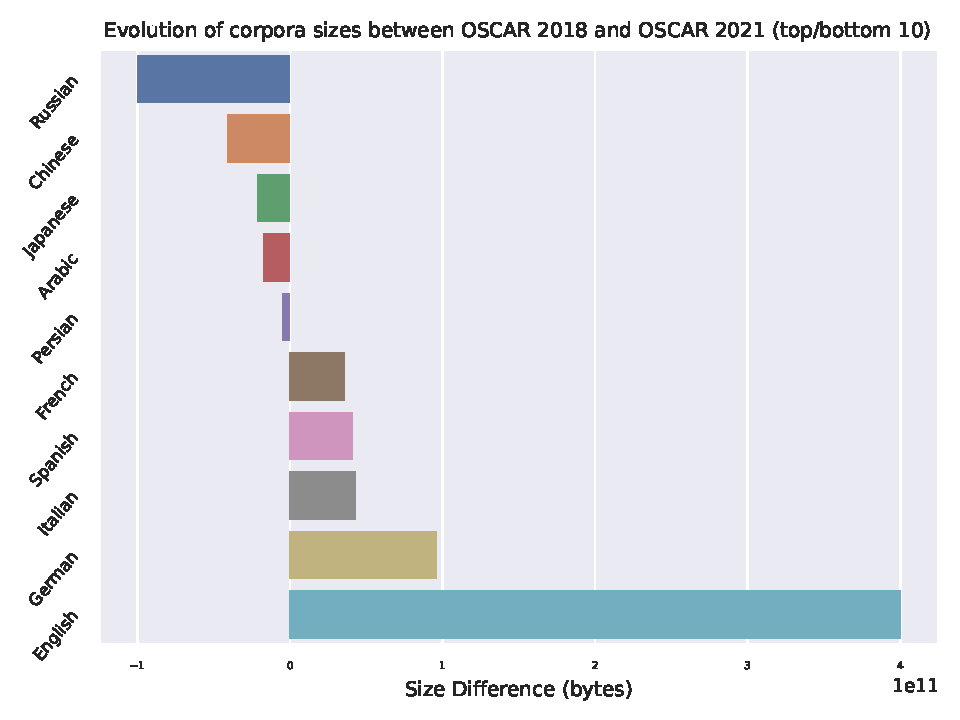
\includegraphics[width=0.75\textwidth, angle=0]{static/media/oscar/ungoliant/size_evo}
    \caption{Comparison of language size (in bytes) between OSCAR 2018 and OSCAR 2021 (top/bottom 5 only). }
    \label{fig:lang-size}
\end{figure}

Results show that already largely represented languages gain more and more data (like the English language, which constituted more than a third of the original OSCAR 2019), except for the Russian language which loses approximately 100Gb of textual content. These results are summarized in Figure~\ref{fig:lang-size}.

However, in a context where the number of languages is very high (higher than 150) and of varying sizes, evolution can't be analyzed via a mere size evaluation. By computing, for each language, the relative size difference between the 2019 and 21.09 releases of OSCAR, less resourced languages do appear, hinting at a better representation of some of them. These results can be found in Figure~\ref{fig:lang-size-pctg}.

Note nonetheless that numerous languages have been omitted from Figure~\ref{fig:lang-size-pctg}, either:
\begin{itemize}
    \item because they were present in the original OSCAR 2019 and are now absent (\textit{Central Bikol} and \textit{Cantonese})
    \item or because they were absent in the original OSCAR 2019 and are now present (\textit{Manx}, \textit{Rusyn}, \textit{Scots} and \textit{West Flemish})
\end{itemize}

Precautions have to be taken when using these corpora and further work has to be done to correctly assess the quality of low-to-mid resource languages in order to better reflect the quality of each corpus to the OSCAR users. Some sub-corpora exhibited either a particularly low number of sentences or just very low quality data, and as such they are not really usable in practice. However, they still account for a language in the total language count of both the original OSCAR 2019 and the new OSCAR 21.09.

\begin{figure}[ht]
    \centering
    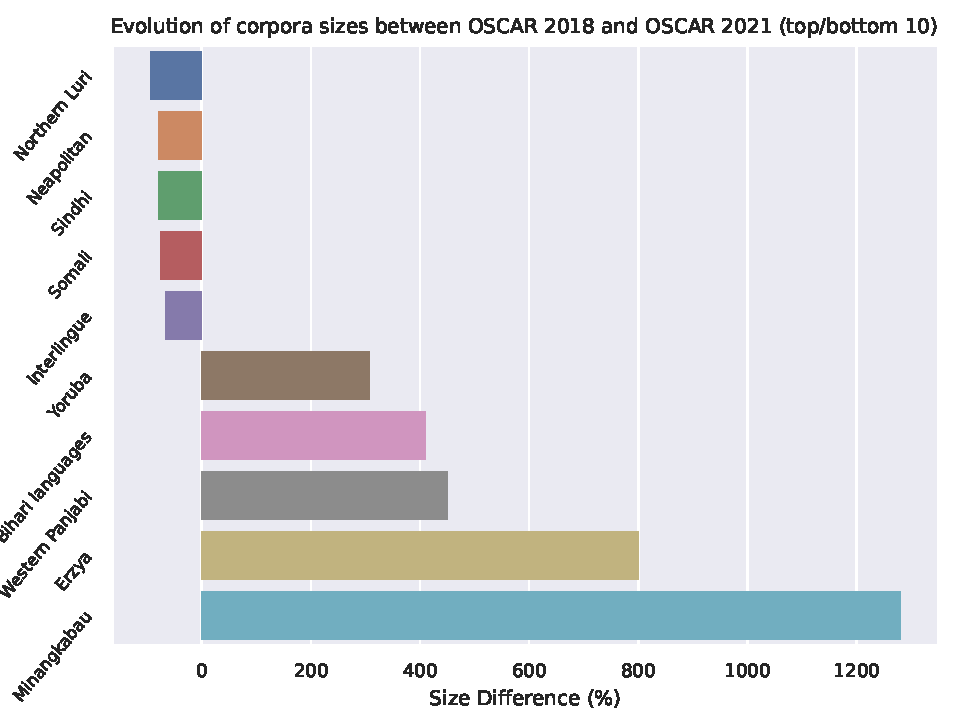
\includegraphics[width=0.75\textwidth, angle=0]{static/media/oscar/ungoliant/size_evo_pctg}
    \caption{Comparison of language percentage between OSCAR 2018 and OSCAR 2021 (top/bottom 5 only).}
    \label{fig:lang-size-pctg}
\end{figure}

\subsubsection{Metadata}

Metadata provides new contextual data that is useful to evaluate the corpus and draw metrics.

The total size of metadata is 1.2TB, ranging from 4Kb to 500Gb, depending on the number of lines. Relative size varies from 100\% to 20\%, diminishing with the textual data size, which is expected.

Our choice of keeping metadata aside from the main content adds some complexity when working with both textual and contextual data:

\begin{itemize}
    \item When trying to get the metadata of given sentence, one has to get the line number $k$, then sequentially (or use a search algorithm since offsets are sorted) look for the record (with offset $o$ and length $l$), where $k \in [o, o+l]$.
    \item Looking for lines corresponding to a particular metadata entry is easier: one has to read the textual file, skipping until the $o$-th line, then read $l$ lines.
\end{itemize}


\subsubsection{Presence of events}

Using a sample of five sub-corpora, we perform a simple search of terms in order to assess and compare the presence of pre- and post- 2018 events and persons in both corpora. Terms and frequency are grouped in Table \ref{tab:word-frequency}.

\begin{table}[t]
    \centering\small
    \begin{tabular}{lrrrr}
        \toprule
        Language                  & Term                  & 2018  & 2021  \\
        \midrule
        \multirow{1}{*}{Arabic}   & Beirut port explosion & 0     & 31    \\
        \multirow{1}{*}{Burmese*} & Min Aung Hlaing       & 387   & 3439  \\
        \multirow{1}{*}{English}  & Obama                 & 30039 & 27639 \\
        \multirow{1}{*}{English}  & Biden                 & 990   & 19299 \\
        \multirow{1}{*}{French}   & Yellow Vests          & 2     & 96    \\
        \bottomrule
    \end{tabular}
    \caption{Comparison of occurrences of news-related terms between OSCAR and our corpus in a sample of 100 Common Crawl shards. For the Burmese language, we use the whole 2018 and 2021 corpus since it is a low resource language. Terms are translated to the target language.}
    \label{tab:word-frequency}
\end{table}

Our corpus keeps around the same number of occurrences for pre-2018 events or public figures such as Barack Obama, while increasing the occurrence of people linked to more recent events (Joe Biden).

We include search terms linked to post-2018 events in French and Arabic which are smaller corpora (resp. 200 and 80 GB), and in Burmese, a mid-resource language (approximately 2GB). We observe a term occurrences evolution that reflects the linked events' timing and importance.

\subsection{License}

This new OSCAR 21.09 corpus is released under a research-only license that is compliant with the EU's exceptions for research in text and data mining. Contrarily to the original OSCAR 2019, no shuffled version of the corpus is distributed, instead we put in place an authentication system that allows us to verify that requests for the corpus come from research institutions. A contact form is also provided for independent researchers so that we can study their particular cases and determine if the utilization of the corpus corresponds to a legitimate research use.

Moreover, the introduction of metadata makes our corpus far more queryable, thus simplifying and speeding up the handling of take-down GDPR requests. For this reason, we release the complete set of metadata under a CC0 public domain license, so that any individual can check if their personal or even copyrighted data is in our new OSCAR 21.09 corpus and make a request accordingly.

\section{Conclusion}

Although the work presented in this particular chapter does not directly address some of the previous concerns raised by \citet{caswell-etal-2020-language,kreutzer-etal-2021-quality}. We do believe that a more efficient, more modular and better documented pipeline is the first step in making the OSCAR project more approachable by other members of the NLP and Digital Humanities communities.

Moreover, we also believe that the addition of metadata to OSCAR is a big step towards improving the quality of its content as it will provide us and other researchers willing to use OSCAR with enough information to better explore, audit, annotate and filter the corpus.

In the next and final chapter of the OSCAR part we will explore the question of document integrity which might be useful for researchers interested in document level tasks and which until now is not respected for Common Crawl records containing multilingual data. We will also continue improving Ungoliant and start using the metadata that we extract from the Common Crawl records to produce the first ever OSCAR annotations.